\documentclass{ctexart}

\usepackage{graphicx}
\usepackage[defaultmono,scale=0.85]{droidsansmono}
\usepackage{amsmath}
\usepackage{amssymb}
\usepackage[hmargin=1.1in,vmargin=1in]{geometry}

\newcommand{\theauthor}{Sparky\_14145}

\input{personal_info/info.tex}

\title{计算机图形 作业六}
\author{\theauthor}

\begin{document}
    \maketitle

    \section{函数流程}

    \subsection{\texttt{Renderer::Render}}

    和作业五基本相同,不再赘述。

    需要强调的两个点是:1. 屏幕平面建议选取 $z=-9$,垂直于 $z$ 轴的平面;2. 最后调用 \texttt{Scene::castRay()} 来获取像素的最终颜色。

    \subsection{\texttt{Triangle::getIntersection}}

    需要完成的部分为:将 \texttt{coord} 等字段设定为正确的结果返回即可。
    
    注意此处:代码中的 \texttt{t\_tmp} 可以直接作为距离,也可以作为光线的参数方程的参数 $t$。

    \subsection{\texttt{Bounds3::IntersectP}}

    对于每一组平行包围面,求出光线所在的直线与它们的交点的参数 $t_1, t_2$,然后令 $t_\mathrm{MS} = \max\{\min(t_1, t_2)\}$, $t_\mathrm{MX} = \min\{\max(t_1, t_2)\}$,则最后如果 $t_\mathrm{MX} > 0 \land t_\mathrm{MX} > t_\mathrm{MS}$,那么光线与这个包围盒相交。

    \subsection{\texttt{BVHAccel::getIntersection}}

    检查当前结点是否是叶子结点。

    如果是叶子,则直接判定光线是否与被包围的物体有交点;否则检查光线是否与自身有交点,如果没有则直接返回,否则依次检查是否与左右子结点有交点,并将交点信息更新为两者中距离较小的那一个然后返回。

    \section{运行结果}

    \begin{center}
        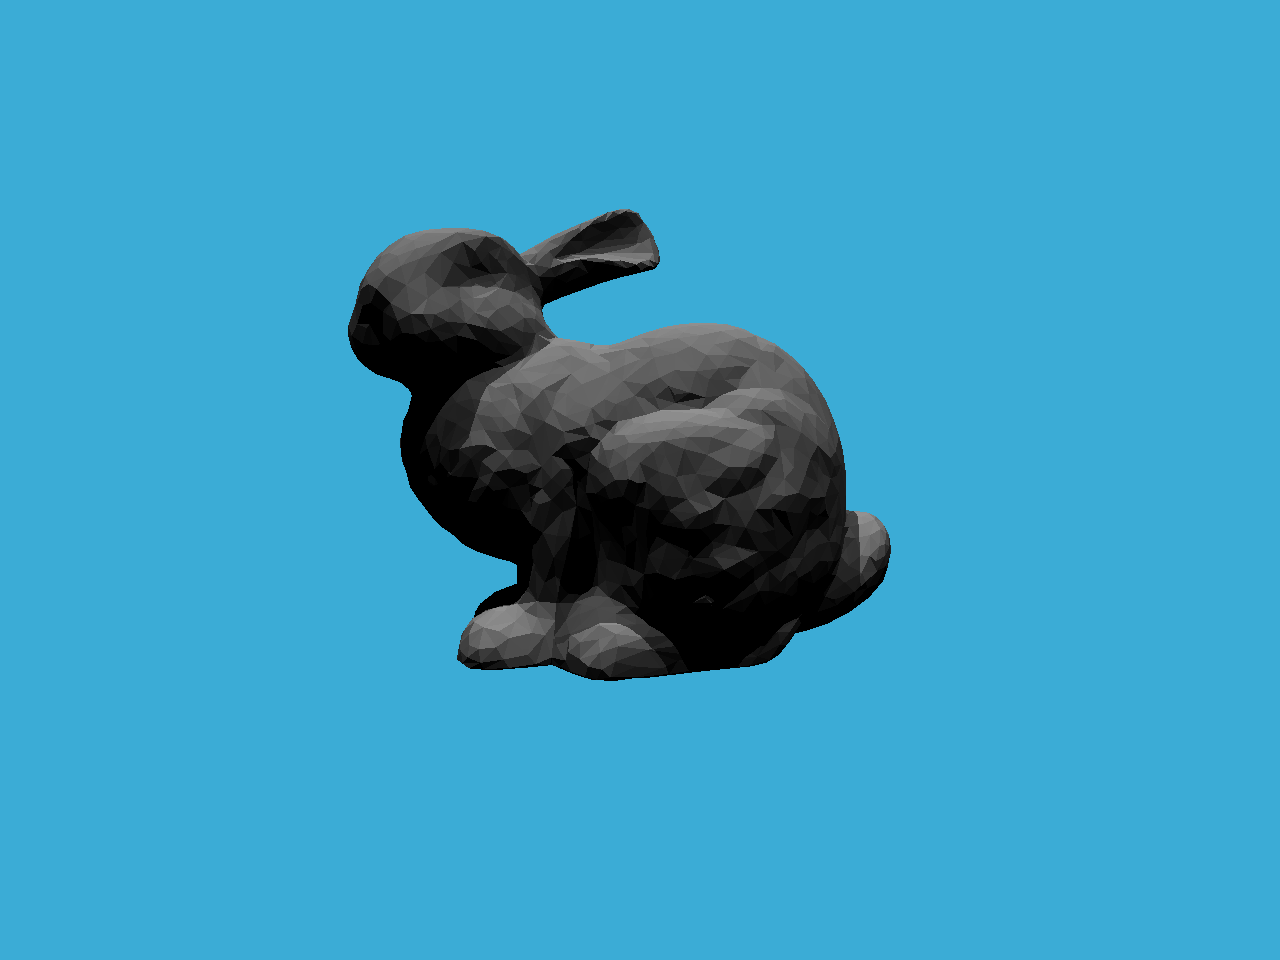
\includegraphics[width=0.9\textwidth]{pics/binary.png}
    \end{center}
\end{document}